% !TEX encoding = UTF-8 Unicode
%%%%%%%%%%%%%%%%%%%%%%%%%%%%%%%%%%%%%%%%%
% Journal Article
% LaTeX Template
% Version 1.4 (15/5/16)
%
% This template has been downloaded from:
% http://www.LaTeXTemplates.com
%
% Original author:
% Frits Wenneker (http://www.howtotex.com) with extensive modifications by
% Vel (vel@LaTeXTemplates.com)
%
% License:
% CC BY-NC-SA 3.0 (http://creativecommons.org/licenses/by-nc-sa/3.0/)
%
%%%%%%%%%%%%%%%%%%%%%%%%%%%%%%%%%%%%%%%%%

%----------------------------------------------------------------------------------------
%	PACKAGES AND OTHER DOCUMENT CONFIGURATIONS
%----------------------------------------------------------------------------------------
\documentclass[oneside, 11 pt]{article}
\usepackage[utf8]{inputenc}
\usepackage[T1]{fontenc}
\usepackage{textcomp}
\usepackage[portuguese]{babel}
\usepackage{blindtext} % Package to generate dummy text throughout this template 
\usepackage{comment}
\usepackage{listings}
\usepackage{xcolor}
\usepackage{hyperref} % For hyperlinks in the PDF

\usepackage{inconsolata}
\lstset{
	language=bash, %% Troque para PHP, C, Java, etc... bash é o padrão
	basicstyle=\ttfamily\small,
	numberstyle=\footnotesize,
	backgroundcolor=\color{gray!10},
	frame=single,
	tabsize=2,
	rulecolor=\color{black!30},
	escapeinside={\%*}{*)},
	breaklines=true,
	breakatwhitespace=true,
	framextopmargin=2pt,
	framexbottommargin=2pt,
	inputencoding=utf8,
	extendedchars=true,
	literate={á}{{\'a}}1 {ã}{{\~a}}1 {é}{{\'e}}1 {í}{{\'i}}1,
}
\usepackage[hmarginratio=1:1,top=32mm,columnsep=20pt]{geometry} % Document margins
\usepackage[hang, small,labelfont=bf,up,textfont=it,up]{caption} % Custom captions under/above floats in tables or figures
\usepackage{booktabs} % Horizontal rules in tables

\usepackage{lettrine} % The lettrine is the first enlarged letter at the beginning of the text

\usepackage{enumitem} % Customized lists
\setlist[itemize]{noitemsep} % Make itemize lists more compact

\usepackage{titlesec} % Allows customization of titles
%\renewcommand\thesection{\Roman{section}} % Roman numerals for the sections
%\renewcommand\thesubsection{\roman{subsection}} % roman numerals for subsections
\titleformat{\section}[block]{\large\scshape\centering}{\thesection.}{1em}{} % Change the look of the section titles
\titleformat{\subsection}[block]{\large}{\thesubsection.}{1em}{} % Change the look of the section titles

\usepackage{fancyhdr} % Headers and footers
\pagestyle{fancy} % All pages have headers and footers
\fancyhead{} % Blank out the default header
\fancyhead[C]{Como Usuários do Linux Ganham Tempo Sem o Mouse} % Custom header text

\usepackage{titling} % Customizing the title section

\usepackage{graphicx}
\usepackage{float}
\renewcommand{\arraystretch}{1.5}
\usepackage{multirow}
\setlength{\parindent}{18pt}
\setcounter{secnumdepth}{0}
\usepackage{tabularx}
	\newcolumntype{L}{>{\raggedright\arraybackslash}X}

\usepackage{xcolor}
\hypersetup{
	colorlinks,
	linkcolor={red!60!black},
	citecolor={blue!50!black},
	urlcolor={blue!80!black}
}
%----------------------------------------------------------------------------------------
%	TITLE SECTION
%----------------------------------------------------------------------------------------

\setlength{\droptitle}{-4\baselineskip} % Move the title up6

\pretitle{\begin{center}\Huge\bfseries} % Article title formatting
	\posttitle{\end{center}} % Article title closing formatting
\title{Como Usuários do Linux Ganham Tempo Sem o Mouse} % Article title
\author{%
	\textsc{Guilherme Bittencourt Bueno da Silva} \\[1ex] % Your name
	\normalsize Universidade Federal do Paraná \\ % Your institution
	\normalsize {gbbs14@inf.ufpr.br} % Your email address
	%\and % Uncomment if 2 authors are required, duplicate these 4 lines if more
	%\textsc{Jane Smith}\thanks{Corresponding author} \\[1ex] % Second author's name
	%\normalsize University of Utah \\ % Second author's institution
	%\normalsize \href{mailto:jane@smith.com}{jane@smith.com} % Second author's email address
}
\date{\today} % Leave empty to omit a date
\renewcommand{\maketitlehookd}{%
	
	%\begin{abstract}
	%\noindent \blindtext % Dummy abstract text - replace \blindtext with your abstract text
	%\end{abstract}
}

%----------------------------------------------------------------------------------------

\begin{document}
	
	% Print the title
	\maketitle
	
	%----------------------------------------------------------------------------------------
	%	ARTICLE CONTENTS
	%----------------------------------------------------------------------------------------
	\section{Resumo}
	Esse material ensina atalhos globais e específicos de aplicações, especialmente no linux mint, porém, muitos comandos específicos de sistemas são utilizados da mesma forma em outras aplicações similares mesmo em outras distribuições do linux ou mesmo em outros sistemas operacionais.
	
	\section{Introdução}
	O uso do shell para realizar atividades repetitivas (ou com algum padrão definido) se provou ser bem mais eficiente que o sistema de apontar e clicar, usado como método principal de entrada de comandos na maioria das interfaces mais usadas atualmente. Apesar do mouse ser muito simples e intuitivo de usar, é comum que usuários mais experientes busquem modos mais rápidos de realizar as mesmas ações. Felizmente, é possível identificar padrões nos principais atalhos do teclado em diferentes interfaces, muitas interfaces, usam o mesmo atalho para ações similares, independente do sistema, e algumas vezes é possível inferir um comando pela inicial da ação a ser realizada.
	
	\section{Atalhos Globais}
	Esse material se limita a focar no Linux Mint, mais especificamente com o ambiente Cinnamon, pois é uma distribuição extremamente fácil de usar para usuário iniciantes e é a distribuição mais acessível para calouros do curso de Ciência da Computação na UFPR. Os atalhos mais importantes do sistema para usuário do shell são atalhos de manipulação de janelas, pois a maneira mais eficiente de usar o shell, geralmente é usando mais de um shell ao mesmo tempo. Os atalhos da tabela \ref{table:1} são os principais atalhos do Linux Mint, com ambiente desktop Cinnamon:
	
	\pagebreak
	
	\begin{table}
		\centering
		\begin{tabular}{|c|p{10.0cm}|}
			\hline
			\bfseries Combinação de teclas & \bfseries Função \\ \hline
			super seta & Expande ou encolhe a janela atual para a direção inserida \\ \hline
			super d & Alterna entre a área de trabalho e as janelas abertas \\ \hline
			alt F4 & Fecha a janela atual \\ \hline
			alt tab & Alterna entre as janelas abertar, começando da janela atual até a janela menos recente\\ \hline
			alt shift & Alterna entre as janelas abertar, na ordem inversa\\ \hline
			ctrl alt backspace & Fazer log off no sistema \\ \hline
			ctrl d & Equivalente ao comando exit, no shell. \\ \hline
			ctrl alt t & Abre um terminal \\ \hline
		\end{tabular}
		\caption{A tabela mostra a combinação das teclas, suas respectivas funções e interfaces onde podem ser utilizados}
		\label{table:1}
	\end{table}

	É importante notar que a criação de atalhos de teclado padrão geralmente é originada usando a inicial da palavra (em inglês) que descreve a função do atalho, por exemplo, em editores de texto, as funções de Negrito, Itálico e Sublinhado, se originam das palavras bold, italic e underline, e portanto seus atalhos são, respectivamente ctrl b, ctrl i e ctrl u. Em alguns editores, quando usados em português, existem dois atalhos para negrito, ctrl b e ctrl n, para servir tanto aos usuários que já usam editores que possuem esse padrão, quanto para usuário que tentam inferir o atalho pelo nome da funcionalidade em português.
	
	Nem sempre é possível inferir o atalho pelo nome, isso porque sua origem é legado de programas antigos que criaram o padrão que é usado atualmente, ou porque já existe uma funcionalidade mais básica que ocupa esse atalho. Nesse caso é possível buscar atalhos com funções similares de outras aplicações e interfaces ou ler o menu de ajuda / manual, ou mesmo pesquisando na internet.
	
	\section{Uso do Sistema}
	Um fluxo de trabalho comum é abrir uma aplicação e carregar um arquivo através dos menus dessa aplicação. O Linux Mint possui uma maneira rápido de realizar a primeira tarefa sem o uso do mouse. Apertando o botão super, o menu de aplicações se sobrepõe à tela e permite ao usuário digitar o nomes de aplicações, menus do sistema e os principais diretórios da home do usuário. Dessa maneira, é possível abrir aplicações apenas com o teclado. Além disso, é possível navegar pela maioria dos menus do sistema usando as setas, "tab" / "ctrl tab" ("shift tab" / "ctrl shift tab" para mover na ordem reversa) e outros atalhos utilizados na maioria das interfaces gráficas. Por exemplo, a interface gráfica do navegador de arquivos do sistema pode ser utilizado completamente pelo teclado. Usando as setas para selecionar arquivos, "enter" para abrir arquivos ou avançar para um diretório, "backspace" para retornar ao diretório pai, "ctrl a" para selecionar todos os arquivos e diretórios, segurar "shift" para realizar uma seleção de multiplos arquivos em sequência e "ctrl w" para fechar. Dessa forma, mesmo quando interfaces exigem que o usuário busque um arquivo através do navegador de arquivos, o mouse não é necessário. Outras interfaces gráficas possuem sistemas de navegação parecido, e muitas vezes, as opções do menu possuem um atalho atribuido, de modo que os usuários que usam o mouse possam se acostumar com os atalhos das opções que utilizam.
	\begin{figure}[h]
		\centering
		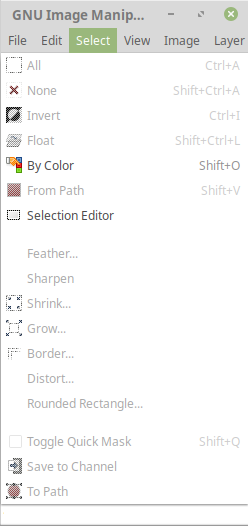
\includegraphics[width=4.0cm]{shotc.png}
		\caption{A figura mostra um exemplo de atalhos referentes às opções de menu.}
		\label{fig:shortc}
	\end{figure}
	
	Outro fluxo de uso comum é buscar um arquivo pelo navegador de diretórios do sistema e abrir o arquivo desejado diretamente com a aplicação escolhida. Isso pode ser feito de maneira mais rápida com o shell, aplicações comuns podem ser iniciadas pelo shell com seus comandos, por exemplo, o comando vlc Downloads/Music abre o programa vlc, com as músicas do diretório (e dos diretórios filhos de) Downloads/Music. Adicionando o caracter '\&', o comando executa no background, sendo possível continuar usando o mesmo shell. Se necessário, é possível redirecionar a saída desse comando para /dev/null para ignorar algumas mensagens que o comando pode retornar durante a execução.
	Para encontrar arquivos, é possível usar o comando find, passando o diretório de partida e uma expressão regular, ou mesmo utilizar das expansões do bash.
	Caso o usuário não conheça o comando para abrir o arquivo desejado, é possível usar o comando gnome-open para abrir o arquivo com uma aplicação inferida através da extensão ou cabeçalhos do arquivo. Devido à existência de outros comandos começados em "gnome-" é recomendada a criação de um alias para esse comando.
	
	\section{Terminal}
	O Shell possui muitas maneiras de facilitar e agilizar tarefas e o sistema possui seus próprios atalhos de navegação entre janelas, mas ainda existem atalhos implementados pelo terminal, a interface gráfica do shell. Como é comum utilizar mais de um shell simultaneamente, o próprio terminal possui a funcionalidade de abrir abas, com o atalho "ctrl shift t". Para alternar entre as abas existentes é possível usar os atalhos "ctrl page up" e "ctrl page down" para, respectivamente, mudar para a próxima aba, ou para a aba anterior. Também é possível navegar pelas abas usando com "alt num", trocando "num" pelo número da aba desejada.	
	
	\section{conclusão}
	É ideal que o usuário busque conhecer os atalhos disponíveis sempre que realizar alguma ação demorada que poderia ser encurtada. A maioria das aplicações possuem atalhos em comum e muitas ainda permitem a criação ou alteração de atalhos. Diferente do mouse, o uso do sistema apenas com o teclado não é tão intuitivo, porém, com um pouco de aprendizado e prática, ele é muito mais rápido e exige menos esforço.


%----------------------------------------------------------------------------------------
%   REFERENCE LIST
%----------------------------------------------------------------------------------------
\end{document}